\documentclass[aps,prb,twocolumn,superscriptaddress,floatfix,longbibliography]{revtex4-2}

\usepackage{minted}
\usepackage{amsmath,amssymb} % math symbols
\usepackage{bm} % bold math font
\usepackage{graphicx} % for figures
\usepackage{comment} % allows block comments
%\usepackage{ulem} % allows strikeout text, e.g. \sout{text}

\usepackage{textcomp} % This package gives the text quote '
\usepackage{algpseudocode}
\usepackage{algorithm}
\usepackage{geometry}
\usepackage{changepage}
\usepackage{enumitem}
\setlist{noitemsep,leftmargin=*,topsep=0pt,parsep=0pt}

\usepackage{xcolor} % \textcolor{red}{text} will be red for notes
\definecolor{lightgray}{gray}{0.6}
\definecolor{medgray}{gray}{0.4}

\usepackage{hyperref}
\hypersetup{
colorlinks=true,
urlcolor= blue,
citecolor=blue,
linkcolor= blue,
% bookmarks=true,
% bookmarksopen=false,
}
\usepackage{xurl}
\usepackage{float}

% Code to add paragraph numbers and titles
\newif\ifptitle
\newif\ifpnumber
\newcounter{para}
\newcommand\ptitle[1]{\par\refstepcounter{para}
{\ifpnumber{\noindent\textcolor{lightgray}{\textbf{\thepara}}\indent}\fi}
{\ifptitle{\textbf{[{#1}]}}\fi}}
\ptitletrue  % comment this line to hide paragraph titles
\pnumbertrue  % comment this line to hide paragraph numbers

% \makeatletter
% \let\c@figure\c@table
% \makeatother

% minimum font size for figurese
\newcommand{\minfont}{6}

% Uncomment this line if you prefer your vectors to appear as bold letters.
% By default they will appear with arrows over them.
% \renewcommand{\vec}[1]{\bm{#1}}

% Allows to rewrite the same title in the supplement
\newcommand{\mytitle}{Efficient rank-based statistic for partially overlapping gene sets}

\begin{document}

\title{\mytitle}

\author{Roc Salvador Andreazini}
\email[]{rocs@stud.ntnu.no}
\affiliation{Department of Computer Science, Norwegian University of Science and Technology, Trondheim, Norway}
\author{Pål Sætrom}
\email[]{pal.satrom@ntnu.no}
\affiliation{Department of Clinical and Molecular Medicine, Norwegian University of Science and Technology, Trondheim, Norway}


\date{\today}

\begin{abstract}
Gene set enrichment analyses use rank-based statistics to test whether related genes are uniformly distributed in an ordered gene list. By testing several gene sets with defined biological functions on gene lists from a biological experiment, one can determine whether specific biological functions are significantly affected by the experiment. The goal of this thesis is to develop efficient algorithms for computing rank-based statistics for thousands of gene sets on tens of thousands of gene lists and use these as a basis for analyzing data from single-cell sequencing experiments.
\end{abstract}

\maketitle
\section{\label{sec:Start}Introduction}

\subsection{Objectives} This thesis aims to develop efficient algorithms for computing rank-based statistics for thousands of gene sets on tens of thousands of gene lists and use these as a basis for analysing data from single-cell sequencing and RNA sequencing experiments.

The current single-cell sequencing analysis landscape does not include rank-based statistics in the data preprocessing steps. This thesis aims to find the differences in the single-cell sequencing analysis when using and not using these algorithms.

\subsection{Background}

\ptitle{RNA sequencing} RNA sequencing (RNA-seq) is a powerful experimental technique for studying gene expression and transcriptomics. It allows researchers to quantify and analyse the RNA molecules present in a biological sample, providing insights into the transcriptional activity of genes.

The main analysis goal in RNA-seq is often to identify differentially expressed genes or transcripts between different conditions or experimental groups. Statistical methods, such as the negative binomial-based methods (e.g., DESeq2, edgeR) or maximum likelihood estimation (e.g., Cufflinks), are commonly used to detect significant changes in expression levels. These analyses provide insights into the genes or pathways upregulated or downregulated under specific conditions.

Once differentially expressed genes are identified, further analyses can be performed to understand their biological significance. Gene ontology (GO) enrichment analysis, pathway analysis, and functional annotation can help elucidate the underlying biological processes, molecular functions, and cellular components associated with the differentially expressed genes.


\vspace{2mm}

\ptitle{Single-cell sequencing} \cite{triumphs-and-limitations-scRNA} Single-cell sequencing (scRNA-seq) examines the sequence information from individual cells with optimized next-generation sequencing technologies, providing a higher resolution of cellular differences and a better understanding of the function of an individual cell in the context of its microenvironment.

These improvements in the technology for sampling expression cells generate some computational problems:
\begin{itemize}
 \item Large datasets: The experiments can capture hundreds of thousands of cells.
 \item Sparse matrices: scRNA-seq experiments generate a result matrix with most zero values due to biological and technological limitations.
 \begin{itemize}
    \item Biological heterogeneity: Not all genes are expressed in every cell, resulting in many zero or low expression values.
    \item Dropout events: Dropout refers to the phenomenon where the expression of a gene is not detected or is detected at deficient levels in a single cell, even though the gene is expressed in reality.
 \end{itemize}

\end{itemize}

\subsection{Methods}

\ptitle{Rank-based statistics} Single-sample Gene Set Enrichment Analysis (ssGSEA) is a computational method used to assess the activity or enrichment of predefined gene sets within individual samples or observations, such as gene expression profiles. It is an extension of the traditional Gene Set Enrichment Analysis (GSEA) that is typically performed on a cohort or population of samples.

SsGSEA aims to determine the relative activity levels of predefined gene sets within a single sample. This approach is particularly useful when analysing gene expression data from individual patients or experimental conditions, where the focus is on understanding the molecular characteristics of a specific sample rather than comparing it to others.

\vspace{2mm}

\label{sec:ks-statistic}
These are the steps followed for the single-sample GSEA, and its corresponding input and output matrices Figure \ref{fig:inout}:

\begin{enumerate}

\begin{figure}[h]
    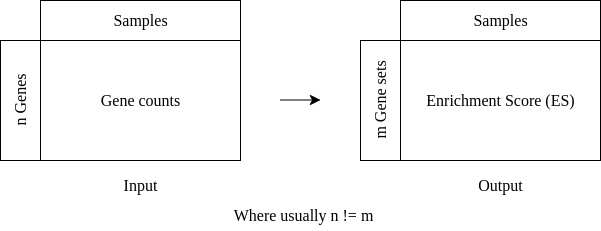
\includegraphics[clip=true,width=7cm]{img/io-gsea.png}
    \caption{GSEA input and output matrices}
    \label{fig:inout}
\end{figure}

\item Normalize the expression matrix.
\item Sort the gene counts for each sample in descending order.
\item Compute the enrichment score. For every sample and gene set, being the score for each sampled gene ($S_i$). For this thesis, the statistic used is a normalized Kolmogorov-Smirnov statistic \cite{diabetes}:
\begin{equation}
S_i = \sqrt{\dfrac{N - G} {G}}
\label{eqn:EPS}
\end{equation}

if the gene is in the current gene set

\begin{equation}
S_i = -\sqrt{\dfrac{G} {N - G}}
\label{eqn:ENS}
\end{equation}

if it's not.

\begin{equation}
ES = \max_{{1 \leqslant j < N}}\sum_{i=1}^{N} S_i
\label{eqn:ES}
\end{equation}

Where $N$ is the number of sampled genes, $G$ is the size of the current gene set

\end{enumerate}
\vspace{2mm}

\ptitle{Linear models} \cite{limma} Linear models are used to analyze gene expression data and identify differentially expressed genes between different experimental conditions or groups. The linear model framework provides a flexible and powerful approach to account for various sources of variation and performs statistical inference.

A linear model is defined as:

\begin{equation}
y = X\beta + \epsilon
\end{equation}

where:

\begin{itemize}
\item $y$ represents the observed gene expression data for a particular gene across different samples.
\item $X$ is the design matrix incorporating information about the experimental conditions or groups. Each column of $X$ represents a factor or covariate associated with the experiment (e.g., treatment, time points).
\item $\beta$  is the vector of coefficients that represents the differential expression effects associated with each factor or condition. Each coefficient $\beta$ corresponds to the effect of a particular factor on gene expression.
\item $\epsilon$ represents the residual error term, accounting for the random variation that the factors in the model cannot explain.
\end{itemize}

The linear model aims to estimate the coefficients $\beta$ and test for the significance of the differential expression effects. This is done through the application of statistical methods, such as hypothesis testing or estimation of effect sizes.

\ptitle{Cell clustering} \cite{clustering} Clustering is a data analysis method that aims to group similar objects while maximizing the dissimilarity between different groups. In single-cell sequencing experiments, clustering is employed to identify distinct cell populations based on their transcriptional profiles. By partitioning the dataset into subsets of cells that exhibit similar gene expression patterns, clustering allows for uncovering hidden structures and relationships within the cellular landscape.

There are several methods for cell clustering:

\begin{itemize}
\item K-means Clustering:
K-means clustering is a partition-based clustering algorithm that aims to divide the data into K distinct clusters. It iteratively assigns each data point (cell) to the cluster with the closest centroid based on a distance metric, typically Euclidean distance. The algorithm recalculates the centroids and updates the assignment until convergence. K-means clustering is easy to implement and computationally efficient but assumes equal-sized and spherical clusters.

\item Hierarchical Clustering:
Hierarchical clustering creates a hierarchy of clusters by successively merging or splitting them based on similarity or distance measures. It can be agglomerative (bottom-up) or divisive (top-down). Agglomerative hierarchical clustering starts with each data point as a separate cluster and then merges them based on similarity, resulting in a dendrogram. Divisive hierarchical clustering begins with all data points in one cluster and recursively splits them into smaller clusters until each data point is in its own cluster. The choice of distance metric and linkage method (e.g., Ward's method, average linkage, complete linkage) influences the clustering results.

\item Shared Nearest Neighbor (SNN) Clustering:
SNN clustering is a graph-based clustering method that constructs a graph connecting cells based on their shared nearest neighbours. It quantifies cell similarity using a distance metric and connects cells with many nearest neighbours. The SNN graph is then partitioned into clusters using community detection algorithms such as Louvain clustering or Markov clustering. SNN clustering captures the local structure of the data, is robust to noise, and can identify clusters of varying sizes and shapes.

\item Graph-based Clustering (Louvain, Leiden, etc.):
Graph-based clustering methods leverage graph representation of the data, where cells are nodes and edges represent relationships or similarities. These methods optimize an objective function, such as modularity, to detect communities or clusters within the graph. The Louvain and Leiden algorithms are popular graph-based clustering approaches used in scRNA-seq analysis. They iteratively optimize the modularity by merging or splitting clusters, aiming to maximize the division's quality.
\end{itemize}

\section{\label{sec:LaTeX} Methods}

\ptitle{gseacc} gseacc is an R package developed for this thesis to run the ssGsea for RNA-seq and scRNA-seq datasets.  It uses the Rcpp library to run C++ code in R. The reason why C++ was chosen is because it offers excellent performance and Objective Oriented programming. The main features of the package are:
\begin{itemize}
 \item Multithreading
 \item Low RAM usage in large scRNA-seq datasets
\end{itemize}

The source code and its corresponding documentation are in \cite{gseacc-github}. There are two different pieces of documentation, one for the package source code (C++) and another one for the R functions that can be accessed while running R.

\subsection{RNA sequencing}

\ptitle{gseacc} For the RNA-seq experiments, \texttt{gseacc} uses the Kolmogorov-Smirnov as the rank statistic (\ref{sec:ks-statistic}). Before running it, the data has to be normalized and sorted. \texttt{gseacc} normalizes the data by first applying an RPM (Rounds Per Milion) normalization for all the samples across the genes, meaning that the sum of the counts in any sample is one million. Then it means-centres the genes across the samples by subtracting the gene's mean expression to every sample.

\begin{figure}[H]
\caption{Pseudocode of ssGSEA function for RNA-seq in \texttt{gseacc}}
\label{fig:gsea-algorithm}
\begin{algorithmic}[1]
\State{$N$ $\gets$ number of sampled genes}
\State{$GS$ $\gets$ number of gene sets}
\For{$k \gets 1$ to $GS$}
    \State{$G$ $\gets$ $geneSet_k$ size}
    \State{$positive$ $\gets$ $\sqrt{\dfrac{N - G} {G}}$}
    \State{$negative$ $\gets$ -$\sqrt{\dfrac{G} {N - G}}$}
    \For{$j \gets 1$ to $S$}
        \For{$i \gets 1$ to $N$}
            \State{$current$ $\gets$ {$0$}}
            \State{$max$ $\gets$ {$0$}}
            \If{$genes_i$ in $geneSets_k$}
                \State{$current$ $\gets$ $current$ + $positive$}
            \Else
                \State{$current$ $\gets$ $current$ + $negScore$}
            \EndIf
            \State{$max$ $\gets$ $max(max, current)$}
        \EndFor
        \State{$results_{ij}$ $\gets$ max}
    \EndFor
\EndFor
\end{algorithmic}
\end{figure}


\ptitle{Limma} The linear model used for the RNA experiment is:

\begin{equation}
y = (CTRL + PSNL + PSL + ADNL + ADL) \cdot \beta + 0
\end{equation}

where Healthy control skin (CTRL), non-lesional psoriasis skin (PSNL), lesional psoriasis skin (PSL), non-lesional atopic dermatitis skin (ADNL) and lesional atopic dermatitis skin (ADL) are the different dataset phenotypes.

\subsection{scRNA-seq}

\begin{figure}[H]
\centering
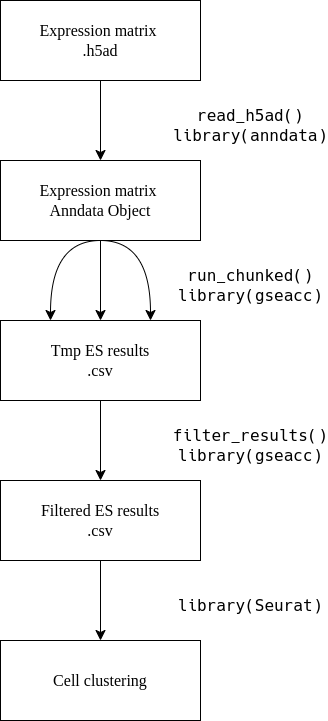
\includegraphics[clip=true,width=4cm]{img/pipeline.png}
\caption{scRNA-seq analysis pipeline}
\label{fig:pixels}
\end{figure}

\ptitle{gseacc} The main challenge to running the Enrichment Score with scRNA-seq datasets is its large size. This is why gseacc implements a function that allows running the GSEA algorithm in chunks. These chunks are obtained by splitting the expression matrix by samples, in the case of \texttt{Anndata} objects, using the \texttt{chunk\_X} function. Since the algorithm is run in different function calls and storing the previous results in the RAM is impossible, different output files are generated. The n most variable gene sets across the samples are obtained by running the \texttt{filterResults} function from the \texttt{gseacc} package that takes all the ES data from the different chunks and computes the sample variability for each gene set. (Figure \ref{fig:chunkedgsea})

The main difference with the RNA-seq experiment in the ssGSEA function (Figure \ref{fig:gsea-algorithm}) is that when a zero value is found, the inner loop stops because the input data for the scRNA-seq is sparse. Since the counts of the samples are sorted in decreasing order, only the null values are ignored.


\begin{figure}[h]
\centering
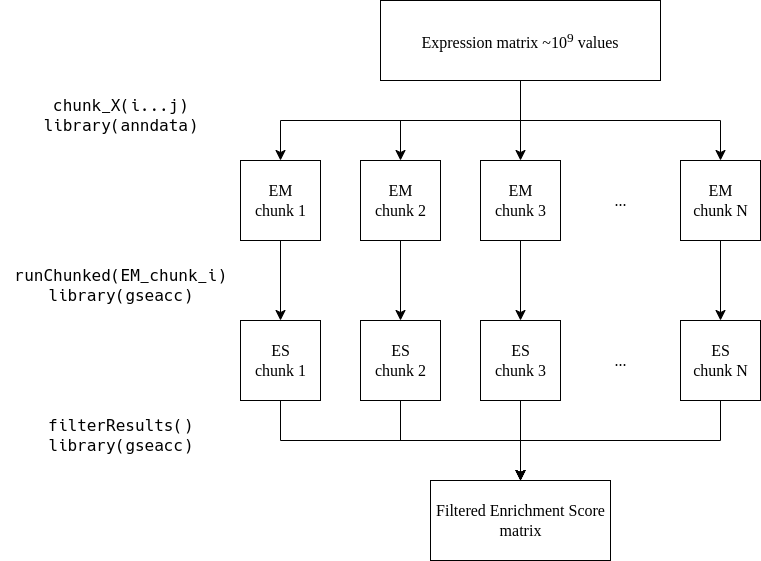
\includegraphics[clip=true,width=7cm]{img/gsea-pipeline.png}
\caption{Chunked ssGsea for scRNA-seq}
\label{fig:chunkedgsea}
\end{figure}


\ptitle{Seurat \cite{seurat-v4} \cite{seurat-web}} The main steps in cell clustering using the Seurat package usually are the following:
\begin{itemize}
\item Scale and centre data: Scale and centre the gene expression matrix to make the gene expression values comparable across cells
\item Principal component analysis (PCA): Use PCA to reduce the dimensionality of the dataset. PCA identifies the principal components that capture the largest data variation sources. These components serve as new features representing the original expression matrix.
\item Find the cell clusters: Construct a nearest-neighbour graph based on the selected principal components, where each cell is connected to its nearest neighbours. Clustering algorithms, such as Louvain or Leiden, are then applied to partition the graph into distinct clusters. These clusters represent putative cell types or states.
\item Reduce dimensionality: Reduce the dimensionality of the clusters using techniques like UMAP (Uniform Manifold Approximation and Projection) to be able to represent the clusters in two dimensions plots.
\end{itemize}

\section{\label{sec:Results}Results and analysis}

All R scripts used for each section can be found on GitHub \cite{thesis-github}.

\begin{table}[H]
\centering
\caption{Resources used to run all the experiments}
\begin{tabular}{ | c | c | }
    \hline
    Processor & Intel® Core™ i5-8250U  \\
    RAM & 8 GB \\
    OS & Ubuntu 23.04 \\
    R version & 4.2 \\
    \hline
\end{tabular}
\end{table}

\subsection{RNA-seq}

\ptitle{The dataset \label{pt:RNAseqdata}} For the RNA-seq experiment, the expression matrix from the GSE121212 experiment \cite{gse121212} was used. It contains 147 samples of 60675 genes. This dataset contains gene counts for different samples of human skin and the following phenotypes:

\begin{itemize}
    \item Healthy control skin
    \item Non-lesional psoriasis skin
    \item Lesional psoriasis skin
    \item Non-lesional atopic dermatitis skin
    \item Lesional atopic dermatitis skin
\end{itemize}

\ptitle{Steps} The Enrichment Score matrix was obtained using gseacc \cite{gse121212-go-es} and analysed using Limma to get the most representing gene sets when comparing different phenotypes.

\begin{table}[H]
\centering
\label{tab:pssolvspsol}
\caption{Scalability for the Enrichment Score computation for the GSE121212 experiment and all the 22962 gene sets from the Gene Ontology. The speedup is the improvement in speed of execution for the execution with one thread.}
\begin{tabular}{ | c @{\hspace{0.6cm}} c @{\hspace{0.5cm}} c | }
    \hline
    Threads & Elapsed time (min) & Speedup \\
    \hline
    \hline
    1 & 398 & 1 \\
    2 & 204 & 1.95 \\
    4 & 111 & 3.59 \\
    8 & 54 & 7.37 \\
    \hline
\end{tabular}
\end{table}

\ptitle{Psoriasis non-lesional vs psoriasis lesional} The results for the most differentially expressed gene sets between the samples with Psoriasis
lesional and Psoriasis non-lesional can be found in the Table \ref{tab:psolvspsonl}.

The most differentially expressed gene set is GO:2000330. This Gene Ontology term is defined as: \textit{Any process that activates or increases the frequency, rate or extent of T-helper 17-cell lineage commitment} \cite{go:2000330}. This cell type is associated with autoimmune diseases such as multiple sclerosis, rheumatoid arthritis, and psoriasis \cite{wiki:Th17}.

\begin{table}[H]
\centering
\caption{Most different expressed gene sets in Psoriasis non-lesional and Psoriasis-lesional. All logFC values in the top 10 are negative, meaning these genes are downregulated in the Psoriasis non-lesional samples and upregulated in the Psoriasis lesional samples. The adjusted p-values of this comparison are low. Therefore, the results are significant. The logFC indicates how much more or how much fewer times the gene set is represented in a log scale in the two phenotypes compared.}
\begin{tabular}{ | c @{\hspace{0.3cm}} c @{\hspace{0.3cm}} c @{\hspace{0.3cm}} c | }
    \hline
    GO term & logFC & AveExpr & Adj. P value  \\
    \hline
    \hline
    GO:2000330 & -282.9675 & 145.89252 & 3.928684e-29 \\
    GO:0048817 & -267.3064 & 94.67299 & 6.638296e-29 \\
    GO:0008973 & -224.9845 & 89.61911 & 6.638296e-29 \\
    GO:0032500 & -220.1325 & 99.53479 & 6.638296e-29 \\
    GO:0002815 & -220.1325 & 99.53479 & 6.638296e-29 \\
    GO:0002805 & -220.1325 & 99.53479 & 6.638296e-29 \\
    GO:0032498 & -220.1325 & 99.53479 & 6.638296e-29 \\
    GO:0006963 & -220.1325 & 99.53479 & 6.638296e-29 \\
    GO:0002807 & -220.1325 & 99.53479 & 6.638296e-29 \\
    GO:0002816 & -220.1325 & 99.53479 & 6.638296e-29 \\
    \hline
\end{tabular}
\label{tab:psolvspsonl}
\end{table}

\ptitle{Control vs Psoriasis non-lesional}

In the case of CTRL vs Psoriasis non-lesional, the most overrepresented gene set is GO:0035373. This gene set is defined as: \textit{Binding to a chondroitin sulfate proteoglycan, any proteoglycan containing chondroitin sulfate as the glycosaminoglycan carbohydrate unit.} \cite{go:0035373}. The expression level of chondroitin sulfate (C6st-1) may be associated with susceptibility to psoriasis \cite{Kitazawa2021}.

\begin{table}[h!]
\centering
\label{tab:ctrlvspsnl}
\caption{Most different expressed gene sets in Control and Psoriasis-lesional. Three upregulated and seven downregulated gene sets are in the Control samples in these cases. The p-values for this test are much larger than in the previous comparison.}
\begin{tabular}{ | c @{\hspace{0.3cm}} c @{\hspace{0.3cm}} c @{\hspace{0.3cm}} c | }
    \hline
    GO term & logFC & AveExpr & Adj. P value \\
    \hline
    \hline
    GO:0035373 & 153.1872 & 157.9633 & 0.000805482 \\
    GO:1904103 & 100.3478 & 129.0386 & 0.001142440 \\
    GO:1904105 & 100.3478 & 129.0386 & 0.001142440 \\
    \hline
    GO:0044595 & -108.4241 & 113.7337 & 0.001350765 \\
    GO:0010420 & -108.4241 & 113.7337 & 0.001350765 \\
    GO:0008689 & -108.4241 & 113.7337 & 0.001350765 \\
    GO:0044596 & -108.4241 & 113.7337 & 0.001350765 \\
    GO:0061542 & -108.4241 & 113.7337 & 0.001350765 \\
    GO:0004395 & -108.4241 & 113.7337 & 0.001350765 \\
    GO:0036194 & -116.3544 & 131.8806 & 0.001350765 \\
    \hline
\end{tabular}
\end{table}

\subsection{Gene set analysis vs gene analysis}

The results in the previous section correspond to what we get when using a rank-based statistic. This section compares the two methods using the clustering \texttt{Seurat} tools.

The two resulting sets of clusters, one obtained from the expression matrix, Figure \ref{fig:rna-expr-clusters} and the other from the ES matrix, Figure \ref{fig:rna-expr-clusters}, have a similar meaning but a really different shape. In the case of the ES cluster, the AD lesional and Psoriasis lesional are far more apart from the rest of the clusters. That is not the case for the expression matrix clusters, where these two sample groups are separated and closer two the rest of the groups. That means the ES clusters make a stronger differentiation between lesional and healthy/non-lesional groups, whether the expression matrix clusters make each individual group more detailed.

The heatmaps, Figures \ref{fig:rna-expr-heatmap} and \ref{fig:rna-es-heatmap}, on the other hand, do have not as substantial differences. The genes upregulated in the lesional groups are downregulated in the healthy/non-lesional groups.

\begin{figure}[h]
\centering
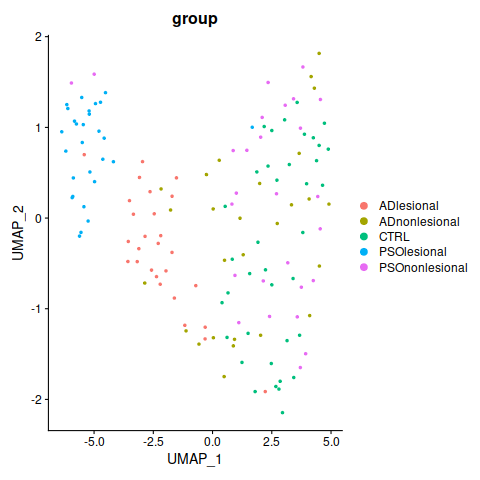
\includegraphics[clip=true,width=7cm]{img/GSE121212-expr-clusters.png}
\caption{Sample clusters from the GSE121212 expression matrix}
\label{fig:rna-expr-clusters}
\end{figure}

\begin{figure}[h!]
\centering
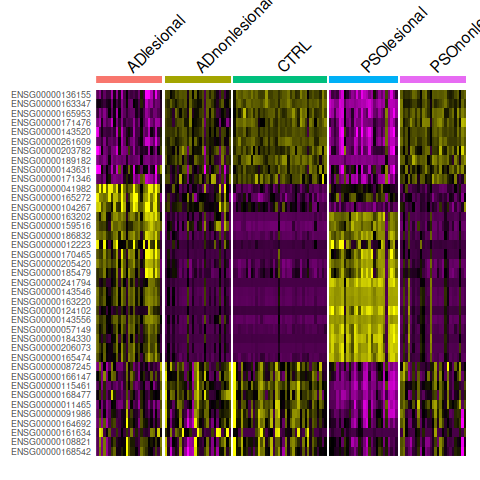
\includegraphics[clip=true,width=7cm]{img/GSE121212-expr-heatmap.png}
\caption{Genes heatmap from the GSE121212 expression matrix. The light yellow cell represents that the gene/gene set is upregulated in that sample, and light purple is downregulated.}
\label{fig:rna-expr-heatmap}
\end{figure}

\begin{figure}[h]
\centering
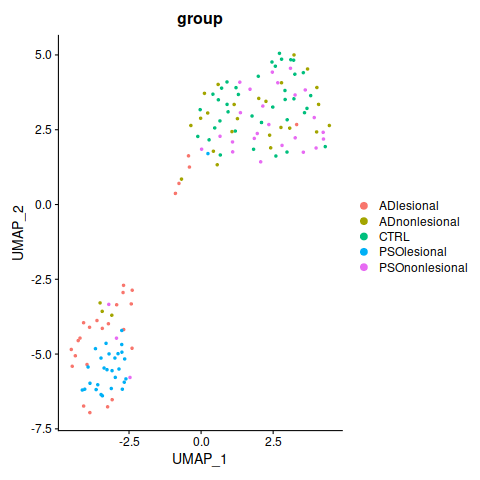
\includegraphics[clip=true,width=7cm]{img/GSE121212-ES-clusters.png}
\caption{Sample clusters from the GSE121212 Enrichment Score matrix}
\label{fig:rna-es-clusters}
\end{figure}

\begin{figure}[h]
\centering
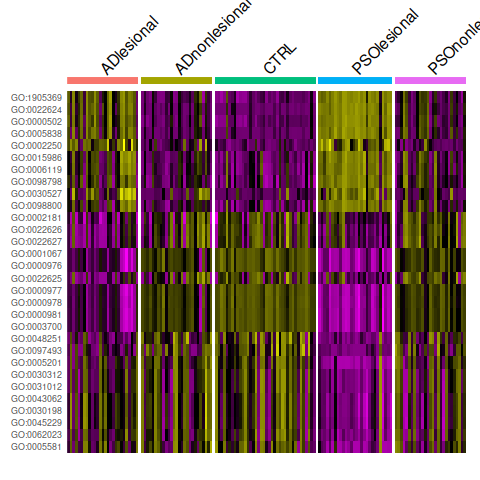
\includegraphics[clip=true,width=7cm]{img/GSE121212-ES-heatmap.png}
\caption{Heatmap from the GSE121212 Enrichment Score matrix}
\label{fig:rna-es-heatmap}
\end{figure}
\subsection{scRNA-seq}

\ptitle{The dataset} \label{seq:scrna-dataset} The dataset used to test the scRNA-seq GSEA implementation consists of $1.9\cdot10^5$ samples (cells) and $2\cdot10^4$ genes from adult human skin. It was extracted from \textit{Developmental cell programs are co-opted in inflammatory skin disease}\cite{healthy}.

It has approximately $10\cdot10^9$ counts, that is, $10^3$ times larger than the RNA-seq dataset (\ref{pt:RNAseqdata}).

\vspace{2mm}

\ptitle{Steps} The first step, as in the RNA-seq experiment, was to run the GSEA. The running time was 16h and 46min using 8 threads, with an average of 4.9 GB of RAM.

The count matrix was split into 100 chunks, and then the Enrichment Score (ES) was computed for all of them. After, these results were filtered by choosing the most variable gene sets across the samples in these same results. Specifically, the first 1000 thousand out of 22736 gene sets were chosen according to the variance results obtained, Figure \ref{fig:scrna-es-stddev}. This first section was run using \texttt{gseacc}.

The next step was to run the clustering algorithms for the ES results. This section was entirely done using the \texttt{Seurat} package. The standard \texttt{Seurat} pipeline was followed. Only the finding of variable features was skipped since they were obtained when filtering the gene sets using \texttt{gseacc}.

\begin{figure}[h]
\centering
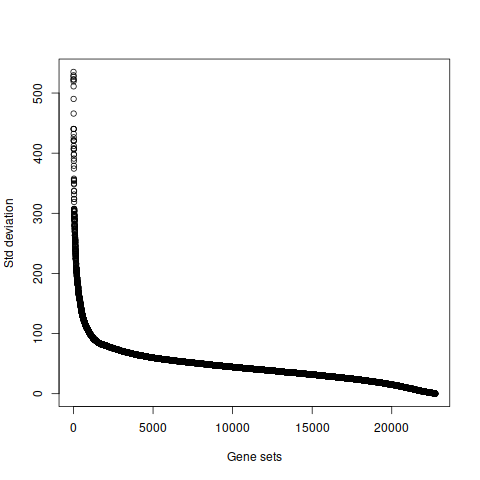
\includegraphics[clip=true,width=6cm]{img/healthy-GO-ES-stddev.png}
\caption{Enrichment Score variance of the gene sets of the Gene Ontology. There are 1034 genes with a standard deviation greater than 100. As seen in the plot, the rest have a similar variability.}
\label{fig:scrna-es-stddev}
\end{figure}

\begin{table}[H]
\centering
\label{tab:vargenesets}
\caption{Top 10 most variable gene sets. As expected, most of these gene sets are related to cell structure since the dataset contains samples of different skin cells. For instance, GO:0005622 is defined as follows \textit{A component of a cell contained within (but not including) the plasma membrane. In eukaryotes, it includes the nucleus and cytoplasm.}}
\begin{tabular}{ | c @{\hspace{0.6cm}} c | }
    \hline
    GO term & Std. dev. \\
    \hline
    \hline
    GO:0005622 & 535.1065 \\
    GO:0043231 & 529.3647 \\
    GO:0005515 & 527.2305 \\
    GO:0005737 & 522.6108 \\
    GO:0043229 & 522.4251 \\
    GO:0043227 & 519.3929 \\
    GO:0043226 & 511.1027 \\
    GO:0005488 & 490.1928 \\
    GO:0003674 & 465.8369 \\
    GO:0031974 & 440.2079 \\
    \hline
\end{tabular}
\end{table}

\ptitle{Cell clustering} To check that the clusters obtained from the ES matrix (Figure \ref{fig:scrna-es-clusters}), the labels of the cells that are present in the count matrix dataset (\ref{seq:scrna-dataset}) were used (Figure \ref{fig:scrna-es-cells}) to be able to analyse the similarities and the differences between the two clustering methods. To have more specific results, a table with the number of overlapping cell samples between the two methods was made, Table \ref{tab:clustercounts}.

\begin{figure}[h]
\centering
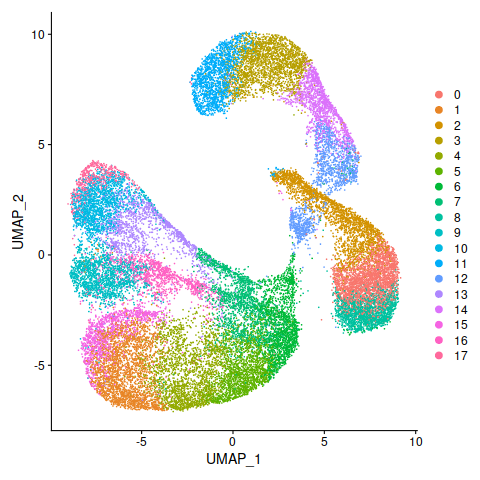
\includegraphics[clip=true,width=6cm]{img/healthy-ES-clusters.png}
\caption{Clusters obtained from the Gene Set Enrichment Score of the scRNA-seq dataset (\ref{seq:scrna-dataset}).}
\label{fig:scrna-es-clusters}
\end{figure}

\begin{figure}[h]
\centering
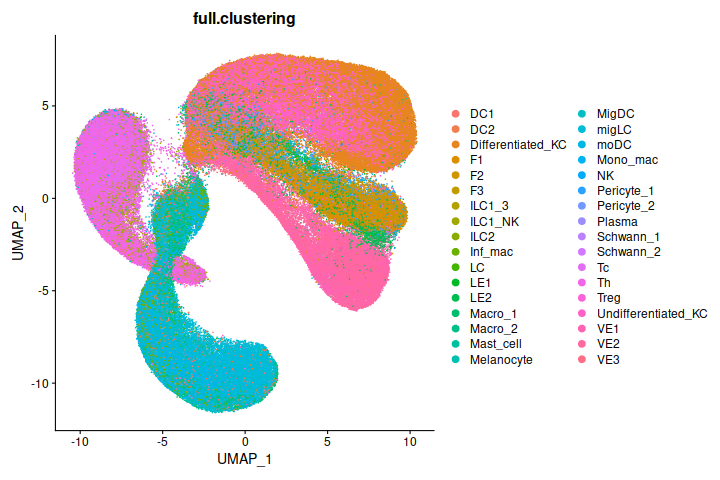
\includegraphics[clip=true,width=8cm]{img/healthy-ES-cells.png}
\caption{Clusters obtained from the Gene Set Enrichment Score of the scRNA-seq dataset, labelled by the cell types already present in the original scRNA-seq dataset (\ref{seq:scrna-dataset}).}
\label{fig:scrna-es-cells}
\end{figure}

\begin{table}[htb]
\centering
\caption{Each table's cell represents the number of cell samples that overlap with the cluster obtained running \texttt{Seurat} from the Gene Set Enrichment Score table and the cell type labels obtained from the original dataset}
\begin{adjustwidth}{-3cm}{-1cm}
\begin{tabular*}{\paperwidth-0.5cm}{| c | @{\hskip 6pt\extracolsep{\stretch{1}}}*{22}{r} |}
    \hline
    Cell type & \multicolumn{22}{c |}{Seurat cluster} \\
 & 1 & 2 & 3 & 4 & 5 & 6 & 7 & 8 & 9 & 10 & 11 & 12 & 13 & 14 & 15 & 16 & 17 & 18 & 19 & 20 & 21 & 22 \\
  \hline
Diff\_KC &   2 &  19 & 6186 & 6765 &  50 & 9490 &  11 &  31 &   6 & 3325 &  27 & 2859 &  13 &  70 &   2 &   3 &   7 &  14 & 2795 &   7 &   4 & 810 \\
  Melanocyte &  11 &  12 &  65 &  53 & 1304 &  63 &   0 &  10 &   1 & 756 &   0 & 1140 &   7 &   5 &   0 & 118 &  86 &   7 &   9 &   0 &   0 &  35 \\
  Undiff\_KC &   2 &   5 & 6818 & 5889 & 124 & 2333 &   4 &  40 &   3 & 3293 &   1 & 2431 &  10 &  25 &   0 &  13 &  17 &  29 & 199 &   0 &   5 & 107 \\
  LE2 &   0 &   0 &  34 &  39 & 2089 &  19 &   1 & 174 &   1 & 264 &   0 & 108 & 123 &   0 &   0 & 648 & 293 &  31 &   3 &   0 &  20 &   4 \\
  F2 &   1 &   0 &   4 &   4 & 1702 &   1 &   3 &   8 &   2 & 483 &   2 & 751 &   2 &   6 &   0 & 573 & 409 &  34 & 177 &   1 &   2 &  95 \\
  LE1 &   0 &   3 &  62 &  24 & 355 &   7 &   0 &  14 &   0 & 211 &   0 & 307 &   3 &   1 &   0 &  29 &  10 &  18 &  28 &   0 &   1 &   0 \\
  F1 &   0 &   0 &   0 &   0 & 2979 &   1 &   0 &   4 &   0 & 229 &   3 & 211 &   1 &   2 &   0 & 3227 & 3440 &   8 &   1 &   1 &   2 &  52 \\
  migLC &  11 &  11 &   0 &   0 &   0 &   0 & 2686 &   4 & 2408 &   0 & 3940 &   1 &   2 & 2626 &   3 &   0 &   0 &   2 &   0 & 283 &   0 &   0 \\
  Th & 8330 & 7163 &   0 &   0 &   2 &   2 &   2 &   0 &   0 &   5 &  25 &  62 &   0 &  32 & 4902 &   0 &   0 &   0 &   2 &  17 &   0 &  73 \\
  F3 &   0 &   2 &   1 &   1 & 1249 &   2 &   2 &  25 &   0 & 117 &   9 &  61 &  13 &   0 &   0 & 860 & 678 &  10 &   2 &   0 &   3 &   0 \\
  VE1 &   6 &   3 &  19 &  19 & 283 &  14 &   1 & 4183 &   3 & 236 &   0 & 186 & 2721 &  16 &   0 & 126 &  44 & 1308 &  23 &   4 & 362 &  88 \\
  VE2 &   0 &   0 &   1 &   0 & 115 &   0 &   0 & 5790 &   0 & 145 &   1 & 118 & 6225 &  14 &   0 &  37 &   9 & 1845 &   1 &   1 & 1196 &  13 \\
  Tc & 4103 & 3608 &   1 &   1 &   0 &   2 &  10 &   0 &   3 &   5 &   8 &  19 &   0 &  35 & 872 &   1 &   1 &   0 &   7 &   1 &   0 &   3 \\
  LC &   2 &   3 &   0 &   0 &   0 &   0 &  39 &   0 & 128 &   0 &  16 &   0 &   0 & 366 &   2 &   0 &   0 &   0 &   0 &  11 &   0 &   1 \\
  Treg & 2412 & 1651 &   0 &   0 &   0 &   0 &  11 &   0 &   8 &   1 &  38 &  12 &   0 &  29 & 1552 &   0 &   0 &   0 &   0 &  14 &   0 &  15 \\
  NK & 164 & 546 &   0 &   0 &   0 &   0 &   0 &   0 &   0 &   0 &   0 &   3 &   0 &   0 &  26 &   0 &   0 &   0 &   0 &   0 &   0 &   0 \\
  Macro\_1 &  23 &   7 &   0 &   0 &  30 &   1 & 1034 &   8 & 1496 &  19 & 824 &  49 &   3 & 2097 &  15 &   2 &   7 &  11 &   1 & 137 &   1 &  16 \\
  ILC1\_NK & 948 & 1173 &   0 &   0 &   0 &   0 &   1 &   0 &   1 &   1 &   4 &   6 &   0 &   1 & 465 &   0 &   0 &   0 &   0 &   1 &   0 &   3 \\
  ILC2 & 216 & 191 &   0 &   0 &   0 &   0 &   0 &   0 &   0 &   0 &   0 &   2 &   0 &   1 &  84 &   0 &   0 &   0 &   0 &   0 &   0 &   0 \\
  ILC1\_3 & 1709 & 758 &   0 &   0 &   0 &   0 &   2 &   0 &   3 &   1 &   5 &   5 &   0 &   3 & 444 &   0 &   0 &   1 &   0 &   2 &   0 &   2 \\
  Macro\_2 &  22 &  11 &   0 &   0 &   8 &   0 & 200 &   4 & 264 &   2 & 178 &  16 &   0 & 509 &   7 &   0 &   1 &   2 &   3 & 190 &   0 &   7 \\
  Plasma &  19 &  33 &   0 &   1 &   2 &   0 &   0 &   0 &   1 &   0 &   3 &   1 &   0 &   0 &  10 &   0 &   0 &   0 &   0 &   0 &   0 &   1 \\
  DC2 &   3 &   9 &   0 &   0 &   0 &   0 &  52 &   0 & 163 &   0 &  15 &   0 &   0 & 427 &   1 &   0 &   0 &   1 &   0 &  52 &   0 &   1 \\
  Inf\_mac &   5 &   3 &   0 &   0 &   0 &   0 & 258 &   1 & 545 &   0 &  47 &   3 &   0 & 245 &   2 &   0 &   0 &   0 &   0 & 653 &   0 &  11 \\
  Mono\_mac &   0 &   1 &   0 &   0 &   6 &   0 & 1527 &   2 & 1402 &   3 & 841 &   3 &   0 & 946 &   6 &   0 &   0 &   1 &   0 & 169 &   1 &   4 \\
  moDC &   4 &   1 &   0 &   0 &   0 &   0 & 4770 &   1 & 3140 &   0 & 2930 &   0 &   0 & 800 &   7 &   0 &   0 &   0 &   0 & 834 &   0 &   3 \\
  MigDC &  20 &   3 &   0 &   0 &   0 &   0 & 625 &   0 & 547 &   1 & 513 &   3 &   1 & 244 &  21 &   0 &   2 &   0 &   0 &  99 &   1 &   0 \\
  DC1 &  36 &  15 &   0 &   0 &   0 &   0 & 177 &   0 & 133 &   0 &  74 &   0 &   0 &  43 &  85 &   0 &   0 &   1 &   1 &  35 &   0 &   4 \\
  Pericyte\_1 &   1 &   5 & 109 &  79 & 2338 &  40 &   0 &  36 &   0 & 497 &   0 & 336 &  13 &   1 &   1 & 843 & 380 &  17 &   3 &   0 &   5 &   1 \\
  Pericyte\_2 &   0 &   0 &   8 &   2 &  32 &   1 &   0 &   0 &   0 &  91 &   0 & 157 &   1 &   0 &   0 &   2 &   0 &   1 &   0 &   0 &   0 &   6 \\
  Schwann\_2 &   0 &   1 &   2 &   1 &  48 &   1 &   0 &   0 &   0 &  27 &   0 &  30 &   0 &   0 &   0 &   4 &   1 &   1 &   4 &   0 &   0 &   0 \\
  VE3 &   0 &   3 &   2 &   0 &  23 &   0 &   1 &  69 &   1 &  22 &   1 &  72 &   5 &  46 &   0 &   0 &   2 & 355 &  20 &   1 &   2 &   4 \\
  Schwann\_1 &   0 &   0 &   0 &   2 &  86 &   0 &   0 &   1 &   0 &  15 &   0 &  12 &   0 &   0 &   0 &  18 &  14 &   1 &   0 &   0 &   0 &   0 \\
  Mast\_cell &  43 &  96 &   2 &   1 &  19 &   2 &   1 &   0 &   1 &  48 &   1 & 315 &   0 &   2 &  24 &   1 &   1 &   0 &   0 &   0 &   0 &   0 \\
  \hline
\end{tabular*}
\end{adjustwidth}
\label{tab:clustercounts}
\end{table}

\section{Conclusions}

\subsection{Limitations}

One of the main limitations of this thesis was computational power limitations since all the programs were run on a middle-end laptop. It mainly affected the cell clustering of Seurat since it required more than 8GB of RAM to run it on the scRNA-seq experiment. On the other hand, having limited resources helped implement the \texttt{gseacc} to be more storage efficient (RAM, not ROM since the chunks take a lot of disk space) and take advantage of all the CPU power using multiple threads.

Another limitation I had for this thesis was not having much knowledge in biology since it limited the amount of analysis I could do after obtaining the results.

\bibliography{report}

\end{document}
